\chapter{Accuracy tests and results}

Every test has been conducted with a camera positioned at 75 centimeters from the ground, with an inclination of 24.6 degrees. Furthermore, the webcam's focal is 519.15 and its field of view is approximatively 90 centimeters wide and almost 40 centimeters tall. Besides, QRCodes are placed on a 3x3 grid and their id is assigned from left to right and from the bottom to the top, as shown in figure \ref{field}. This numbers are not only the id corrisponding to the QRCode but each number indicates where QRCodes are positioned into this field.

\begin{figure}[hbt]
    \centering
    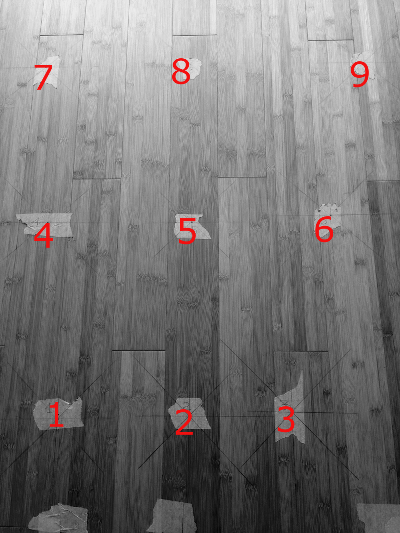
\includegraphics[scale=0.4]{img/field.png}
    \caption{QRCode's grid system. \label{field}}
\end{figure}
\newpage

Moreover, in order to increase the number of tests using the same resources, three pictures for each angle was taken in every location. The orientations used range from 0 to 315 degrees with an increment of 45 degrees in each step. Therefore, these tests was made on a basis of 216 pictures.
\newline
The positions of every marker was measured and they were hard-coded into the program in order to run the proposed software. As can be seen, Table \ref{qrpos} contains the x and y coordinates, in centimeters, for every QRCode's id.


\begin{center}
	\label{qrpos}
  \begin{tabular}{ | l | l | l |}
    \hline
    id & pos\textunderscore x & pos\textunderscore y \\ \hline
    1 & 18.5 & 22 \\ \hline
    2 & 19 & 0 \\ \hline
    3 & 20 & -18 \\ \hline
    4 & 54 & 28 \\ \hline
    5 & 54 & 0 \\ \hline
    6 & 54 & -28 \\ \hline
    7 & 91 & 31 \\ \hline
    8 & 91 & 0 \\ \hline
    9 & 91 & -37 \\ \hline
  \end{tabular}
\end{center}

Therefore, running the algorithm with this configuration, showed that maximum error on angle's calculation is a little more than 8 degrees, although, as can be seen in figure \ref{anglchart}, in most cases the uncertainty is about 2 degrees, which is clearly promising. Along with the above results, the maximum error on the Y coordinate estimation is near to 5 centimeters. However, as can be seen in figure \ref{xchart}, usually it can be found between two and three centimeters. The shape of the chart in \ref{ychart} graph appears strange comparing with the one for X. However, due to the fact that the error is Gaussian distributed on this type of system, this chart shows only the left queue of the distribution while it can be assumed that the right part has to be very similar. As opposed to the above result, experiments showed that estimation on X can have an error of almost 20 centimeters. Furthermore, this problem is present only in 8 images which contained a QRCode very near to the borders of the field of view and with a measured angle between 135 and 225 degrees, in addition those images were affected by a very bright sun light. This implies that, due to the nature of this error, a nearer camera, as the one of a walker which moves forward to the direction of the QRCode, would reduce those problem by sending more data and the results might converge to the error between the 8 and 10 centimeters that figure \ref{xchart} shows\footnote{All the raw data are available in appendix.}.

\begin{figure}[hbt]
    \centering
    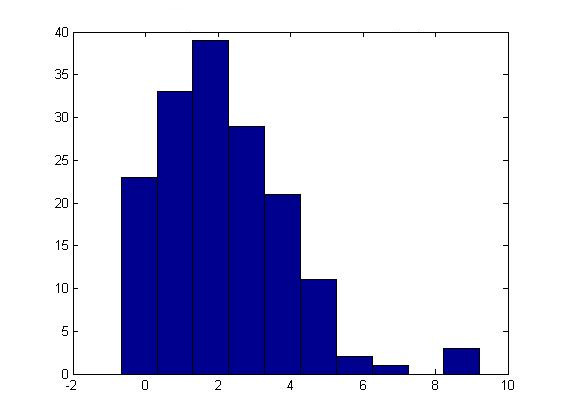
\includegraphics[scale=0.3]{img/chartangl.jpg}
    \caption{Angle estimation histogram\label{anglchart}}
\end{figure}

\begin{figure}[hbt]
    \centering
    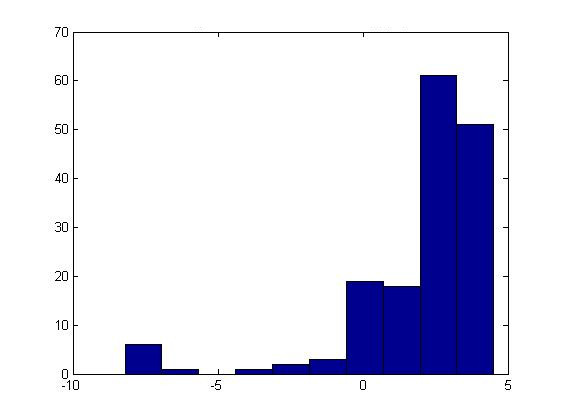
\includegraphics[scale=0.3]{img/charty.jpg}
    \caption{Y estimation histogram\label{ychart}}
\end{figure}
\begin{figure}[hbt]
    \centering
    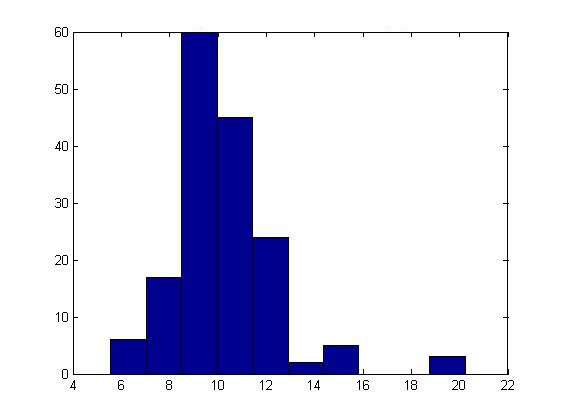
\includegraphics[scale=0.3]{img/chartx.jpg}
    \caption{X estimation histogram\label{xchart}}
\end{figure}



